\chapter{SQLの本をどう選ぶ?}

SQLを学ぼうとするとき、はず、参考書を探すというのはよくあることです。ですが、署名にSQLとついた本を書店で眺めたり、Amazonあたりのネット通販で眺めたりしたとき、どの本を手に取っていいか分からなくなることがあります。

本書では、最初に、SQLを学ぶための本の選択の仕方について記載します。

\section{SQLの本とRDBMSの本は違う}

たとえば、AmazonでSQLをキーワードに和書を検索したら、どのくらいの本が出てくるのでしょうか。2019年3月現在で、和書、洋書、Kindoleを問わずに検索すると、1000種類以上の検索結果が出てきます。

この数では、SQLそのものを学ぶために、どの本を手に取ったらいいか分からなくなります。署名だけで買ってみると、SQLについては全くあっ枯れていない本を引き当ててしまうこともあります。

なぜこのような混迷したことになっているか、というと、SQLという単語が署名につく本には、データベースを操作する言語としてのSQLそのものについて書いてある本と、操作にSQLを使うことができる、リレーショナルデータベース実装の取り扱いについての本と、両方が含まれるためです。

このような混乱を招くのは、SQLを使用することができるリレーショナルデータベースの実装で、書籍が出るくらいメジャーなものは、なんとかSQL,もしくはSQLなんとか、という名前がついていることです。単独で書籍が出るものだと、Microsoftの製品のSQL-Serverや、Oracleに吸収されたMySQL ABのMySQL、PostgreSQLがあります。また、PHPなどに組み込まれている、ソフトウェア組み込み用のデータベースのSQL-Liteというものもあります。

もちろん、なんとかSQLでないリレーショナルデータベースもあります。有名なところでは、Oracle,DB2といった商用データベース、オープンソースだと、FireBirdや、MySQLからフォークした、MariaDBなどがあります。

\subsection{SQLの本}

書名で、SQLの前にも後にもなんとかと付かない本は、SQLそのものについて記述した本になります。たとえば、はじめてのSQL、SQL入門、というタイトルの本は、間違いなく、SQLそのものについて、考え方や書き方の説明をしている本です。

ここでいう、SQLそのものとは、たとえば、SELECTによる検索、CREATEによるテーブルの生成、UPDATEやDELETEによるれこーどのそうさなどについて書いてある本ということです。つまり、SQLという言語の解説書は、おおむね、SQLの前後になんとかとつかない署名を採用しています。

とはいえ、当然ながら、例外というものがあります。それは、特定データベース製品のためにSQLを拡張した言語の入門書は、なんとかSQL、という名前で、その拡張した言語を説明することがあります。

この例として、Oracleが、データベースの自社製品であるOracleのためにSQLを拡張した言語、PL/SQLの解説書が挙げられます。PL/SQLという言語の入門書は、当然、PL/SQLという言語名を、署名に織り込んでいます。

同じように、Microsoftのデータベース製品、SQL-ServerのためにSQLを拡張した言語、Transaction SQL(T-SQL)を解説する本は、T-SQLという言語名から署名を取っているでしょう。そのほかにも、Salesforceが自社SaaSデータベースの操作のためにSQLを拡張した言語は、SOQLという名前です。この言語の解説書が出るときは、SOQLという言語名が署名に付くこととなります。、


\subsection{RDBMSの本}

署名に、リレーショナルデータベースのプロダクトの名前が付いている本は、おおよそ、そのデータベースのインストールや運用、管理、バックアップ取得、などオペレーションの入門書となります。

MySQL入門、PostgreSQL入門、というような署名は、MySQLやPostgreSQLといった、データベースプロダクトのオペレーションについて解説した本です。メンテナンスに必要なコマンドとしてSQLについてこうをさいていることはありますが、SQLについて詳細な説明はありません。

これらの本は、データベースをインストールしたり運用したりする、サーバエンジニアやデータベースアドミニストレータに向けた本です。そのため、SQLを学ぼうという人のための本とは、役割が異なります。


\section{どんなSQLの本を選べばいいのか}

では、言語としてのSQLを学ぼうというときに、どのようなSQLの本を選択すればよいのでしょうか。筆者の個人的な見解を交えつっつ、簡単にまとめてみます。

大型書店では、立ち読み用のコーナを切歯していることが増えました。ですが、そこで、置いてある本の内容をすべて読破するわけにもいきません。どのようなところに、注目すればよいのでしょうか。

\subsection{よさそうな入門書を判断するポイント}

筆者がSQLの入門書を選ぶと木、どのようなところを見るかを節瞑します。ただし、これは筆者の見解であり、特定の書籍を持ち上げ、またはおとしめるものではありません。

SQLの入門書を判断するポイントは、テーブルとレコード、アトリビュートという概念を、どう説明しているかだと、筆者は考えています。

多くの入門書では、テーブルは表計算ソフトの表のようなもの、レコードが行でアトリビュートが列、というような説明をされていることが多いです。筆者の見解として、このような説明をしている入門書は、あまりおすすめしません。
テーブルが表であるというイメージが付いてしまうと、複雑なクエリを書いたりするときに、レコードとレコードの関係がうまくイメージができない、というのが筆者の見解です。

では、どのような説明をしている本がよいのでしょうか。それは、テーブルを丸でかこった空間で表し、レコードをその中のどこかにあるものとして表現している本です。テーブルとレコードを、このような表し方をしている本だと、おすすめできます。

\begin{figure}[htbp]
	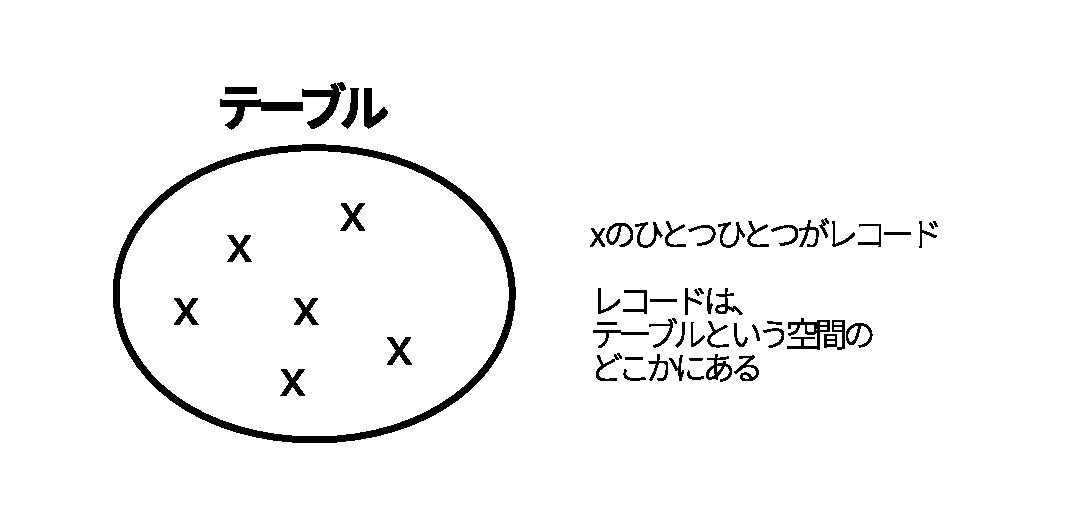
\includegraphics[width=12cm,clip]{draw/table.eps}
	\caption{テーブルとレコード}
	\label{fig:animals_kinds_er}
\end{figure}



\subsection{SQLをより深く学ぶために}

SQLが何をやっているのかをより深く理解したくなったときは、数学の集合論と命題論理を学ぶことをおすすめします。

SQLのテーブルは、集合論でいうところの集合に相当します。そして、SELECTという操作は、命題論理で言うところの命題であり、集合論的な見地での関数に相当します。

本書では数学的な厳密さには立ち入りませんが、必要となったときは、集合論の扉を開いてみる、ということを覚えておいていただければと思います。

